%!TEX root = main.tex

\subsection{Data collection}

Acquiring the required data for this project in itself was quite challenging. A part of the data can be downloaded from the IMDb website\cite{IMDbInterfaces}. This data does not include actor gender, movie plot or box office values. To determine the gender, we used the list of known professions for every person. If they are known for being an actor, they are assigned the label "0", representing male. Actresses are assigned the label "1", representing female. Some people in the dataset have never acted, for example directors or producers. They are removed from the data. There is no way to find the movie plot in the datasets, so we had to find an external source. One alternative is to use webscraping on the IMDB website. We tried doing this but quickly realized that it would not be possible for us to wescrape all the movie plots, because they stop responding to requests after a particular limit in a given time period. We were able to get about 9,000 requests per hour. Since the dataset includes about 500,000 movies, this was not a good solution. It was also not possible for us to know if there were other rate limits e.g. 50,000 requests per day. Instead we used the OMDb API\cite{OMDb} to retrieve the movie plots. Using this API, we were able to get all the plots in 1 hour and 43 minutes. Our original idea was to also make a prediction on the box office value. After using the OMDb API to also find the box office values we saw that only 6381 movies have this value. We do not believe this is enough data to make proper predictions, so we did not use this data. Instead we decided to generate a prediction for the IMDb user score because this value is available for all the movies in our dataset.

One notable challenge was that the data from IMDb is updated every day with new information. This means that you might not get the same result from the search engine as we did when you perform a search. We downloaded the data several times but at one point we noticed that the data can be corrupted, i.e. a lot of information was missing. There seems to be some "luck" involved in the download process. Some days none of the actors have birth years which means that the search engine will not work, other days the ratings were missing. To get the results in this report we used the version of data from the 6th of March 2020. The data from OMDb was only downloaded once on the 12th of March 2020.



\subsection{Preprocessing}

The data from IMDb includes a lot of information we don’t need and it also has missing values. It is split over several files, e.g. \textit{title.basics.tsv} and \textit{title.ratings.tsv}. Every person in the dataset has a unique id, name, birthyear, deathyear, a list of primary professions and a list of titles they are known for working on. We replace the primary profession list with a number indicating the gender. We remove people who are dead or who has never been an actor or actress before. There are also some people who are actors but not known for any titles. They are also removed because we need that information to calculate a score. These steps reduce the number of people from 9.9 million to 200 thousand.

The data in the \textit{title.basics.tsv} file is an id, type, well known title, original title, adult, start year, end year, runtime, and a list of genres. The only relevant information for our project is the id, type and list of genres. The type is used to decide if we should keep it. We are only interested in looking at movies, represented by "movie" or "tvMovie" in the data. Shorts are typically news segments which would not be a good indicator of movie performance. If we included tv series then the actors in them would have inflated scores because there could be over 100 episodes for a given series. That would show that the person is good at that specific role, but not represent how well he or she can adapt to a new role. The runtime is not used in our system because it is missing for most of the titles. Some movies are missing the genre list and are thus removed because it is a mandatorily required for the system. This reduces the number of titles from 6.5 million to 580 thousand. This might seem like a lot, but most of it is because the data includes separate entries for each season and episode for every TV series. In this step we also use the plot data from the OMDb API. Movies without the plot information are removed. This reduces the number further to 212 thousand.

The movie ratings are in the \textit{title.ratings.tsv} file from IMDB. The format is id, average rating and number of votes. Any title removed from \textit{title.basics.tsv} is also removed from this data. The \textit{title.principals.tsv} file contains a list of the most important people for each title. The fields are title id, ordering, actor id, category, job, characters. We use this information to determine what actors have worked together. We only look at the titles with id which was not removed in the previous step, and the ordering, category, job and characters fields are dropped because they provide no relevant information to us.

The information from the ratings and principals files are combined to create a actor to actor relationship graph. Each node in the graph is an actor. Edges between nodes indicate that the two actors have worked together. The value of the edge is used to store how positive the connection is. If the movie they worked together on is highly ranked by users of IMDb then the value will be low. If the user rating is low then the value is high. 



\subsection{Ranking algorithm}

The ranking algorithm is used to give a score to the actor groups. The score is given as a number between 0 and 10, where a higher score indicates a higher rank. The final score is a combination of three scores. We call the first one the genre score. It is calculated based on the actors previous performance in that particular genre. The second score is the similarity score. It is calculated from the plot summary of the movies a person has acted in. The third and final score is the relation score between the actor and the other actors in the group. The final score is the weighted average of these scores. The weighting is chosen by the system based on how many relationships are found within the group.

\subsubsection{Selecting actors}

The first part of the ranking algorithm is to find every actor matching the search query. This is done using SparkSQL and Spark Dataframe operations as shown in listing \ref{CodeActorSelection}. The user supplied descriptions are read from the \textit{search\_actors} list.

\begin{lstlisting}[float=h!, language=Python, caption=Actor selection in PySpark implementation, label=CodeActorSelection, numbers=left]
candidate_sql = "SELECT nconst, genre_score, tconst FROM Actors WHERE age >= {0} AND age <= {1} AND gender= {2}"
candidates = []
for i, desc in enumerate(search_actors):
    # Select actors based on the actor description
    cand = spark.sql(candidate_sql.format(desc[1], desc[2], 1 if desc[0] == "Female" else 0))
    # Create condition that will only select actors with all of the genres.
    genre_condition = cand.genre_score.contains(search_genres[0])
    if len(search_genres) > 1:
        for genre in search_genres[1:]:
            genre_condition &= cand.genre_score.contains(genre)
    cand = cand.filter(genre_condition).withColumn("tconst", convert_to_arr(cand.tconst))
    # Actor score calculation omitted.
    candidates.append(cand)
\end{lstlisting}

\subsubsection{Genre score}

To calculate the genre score we need to convert the movie data to a different format. The raw data we use are the ratings, principals and title files. They are read by a MRJob script which calculates the weighted average for each genre for each actor. The weights are the number of votes for that title. If an actor has acted in two movies, one with the genres "Adventure" and "Drama", the other with the genres "Adventure" and "Action" then the actor will have genre scores for the genres "Adventure", "Drama" and "Action". The "Drama" and "Action" scores will be the rating that those movies have on IMDb. The "Adventure" score will be a weighted average of both ratings. Assuming that the first movie had 10 votes and a rating of 9, and that the second movie had 90 votes and a rating of 3 then the "Adventure" score is $$\frac{10}{10+90}\cdot9+\frac{90}{10+90}\cdot3=3.6$$

Our initial version of the genre score did not consider the number of votes. We quickly realised that a lot of movies have very few votes, and that those movies often have a high rating. It would be hard to set a threshold of minimum number of votes because it could exclude new actors who might not have a lot of experience.

The MRJob consists of one mapper and two reducers. The mapper reads each line and yields the data such that when reducing all of the information for a movie is available on the same line. An example of what is returned if the input line belongs to ratings.tsv is showed in code listing \ref{GenreScoreCode1}. In the first reducer the format is changed from being all of the information about a movie to yielding the information relative to the actor. If for example there are three actors in a movie, then there will be three yield calls with the genres and the rating of the movie. Some of the code is shown in listing \ref{GenreScoreCode2}. The final reducer operates on the actor information and calculates the weighted average of the scores. A snippet of this is shown in listing \ref{GenreScoreCode3}.



\begin{lstlisting}[float=h!, language=Python, caption=Genre score mapper, label=GenreScoreCode1, numbers=left]
def mapper_collect_title(self, _, line):
        values = line.split("\t")
        # ratings.tsv
        if len(values) == 3:
            yield values[0], ["rating", (values[1], values[2])]
            return
        # principals.tsv
        if values[1][:2] == "nm":
            yield values[0], ["actor", values[1]]
            return
        # title.tsv
        yield values[0], ["genres", values[1].split(",")]
\end{lstlisting}



\begin{lstlisting}[float=h!, language=Python, caption=Genre score first reducer, label=GenreScoreCode2, numbers=left]
def reducer_title(self, key, values):
    # Generation of the genres object omitted.
    genre_ratings = {genre: rating for genre in genres}
    for value in values:
        if value[0] == "actor":
            yield value[1], genre_ratings
\end{lstlisting}

\begin{lstlisting}[float=h!, language=Python, caption=Genre score final reducer, label=GenreScoreCode3, numbers=left]
def reducer_actor(self, actor_id, values):
    # Generation of the scores object omitted.
    avg_scores = {}
    for key in scores:
        votes = sum([float(score[1]) for score in scores[key]])
        s = sum([float(score[1])/votes * float(score[0]) for score in scores[key]])
        avg_scores[key] = round(s, 4)
    yield actor_id, "{}\t{}".format(actor_id, avg_scores)
\end{lstlisting}



\subsubsection{Similarity score}
The similarity score is calculated by comparing the summary plot given as input by the user and the summary of the movies acted by the actors with high genre scores. For this purpose, we tried the following methods:

\begin{itemize}
    \item \textbf{Cosine similarity using Tf-idf:}The cosine similarity is the cosine of the angle between two vectors. In text analysis, each document can be represented as a vector. Mathematically, cosine is the dot/scalar product of two vectors divided by the product of their Euclidean norms. The lesser the value of cosine, the lesser the similarity between the two documents and vice versa. Tf-idf is short for term frequency-inverse document frequency and is often used in information retrieval and text mining. The text in the documents are tokenized and lemmatised, then tf-idf measures the frequency of each word occurring in a document, and comes up with a tf-idf matrix whose similarity is then computed. This method depends very much on the number of words in a document. Which is why this was a bad choice for our task, since our plot summaries are small, with very few words. Nevertheless, we tried implementing this, but the results were highly dissatisfactory.    
    \item \textbf{Word2Vec: }Word2Vec as the name sounds is a neural network that maps words to a vector and then analyses them mathematically. Its purpose is to cluster the vectors of similar words together in a vector space. That is, it detects similarities mathematically. Word2vec creates vectors that are distributed numerical representations of word features, features such as the context of individual words. This  method  was  highly  promising  but  yielded  poor  results since it was computing word-wise similarity while we needed sentence-synonymity.
    \item \textbf{Tensorflow model from Google: }The model \cite{TFHubModel} available in the TensorFlow Hub is also a form of word2vec model but is instead trained and optimized for greater-than-word length text, such as sentences, phrases or short paragraphs. This perfectly matched our criteria and gave excellent results. This model would return a value between 0 and 1 which we multiplied by 10 to normalise it like the genre score.
\end{itemize}

To show the problems we faced while using the tf-idf method to calculate the plot similarities, some of the top results are included in table \ref{tab:tfidf}. The text column indicates whether or not the plot is similar to the themes found in the Interstellar plot. Plots that include themes like aliens, global disasters and space travel are marked by "Ok". The two plots marked "Not ok" are romance related. The complete plot summaries are included in section \ref{sec:appendixB}, Appendix B - Movie plots. The first problem is the similarity score which differ a lot between some plots while other plots are close. The first plot belongs to Interstellar and it is expected to be first with a similarity close to one. Because the following plot similarity is approximately 0.12 then the original cast of Interstellar will be given a much higher similarity score compared to every other actor. The second problem is that two movies which are not similar in the plot are included in the top 10 plot similarities. This means that actors of movie 7 and 9 are given an advantage over actors in movie 10 even though they have acted in a movie with a less similar plot. If we had used this method to adjust the actor scores then the result would have been less correct.
\begin{table}[H]
    \centering
        \begin{tabular}{ |c|c|c| } 
            \hline
            \textbf{Order} & \textbf{Score} & \textbf{Text} \\ 
            \hline
            1 & 1.0 & Ok \\
            2 & 0.12166245 & Ok \\
            3 & 0.11172818 & Ok \\
            7 & 0.09751986 & Not ok  \\
            9 & 0.09095107 & Not ok \\
            10 & 0.08666907 & Ok \\
            100 & 0.048099644 & Not ok \\
            \hline
        \end{tabular}
        \caption{Plot similarity using tf-idf}
        \label{tab:tfidf}
\end{table}
    
Similarly we can inspect the result of the Tensorflow model scores shown in figure \ref{tab:tfsim}. This model somewhat solves the problem in the large difference between the similarities. The first and second result are now closer together. In addition we see that the model is a lot better at ranking the plots based on theme. Every movie in the top 10 list is very similar in the plot, and even after looking at the top 100 movies the plots are similar. Some of the movies do not contain the space themes anymore, but they are still related to a global disaster.

\begin{table}[H]
    \centering
        \begin{tabular}{ |c|c|c| } 
            \hline
            \textbf{Order} & \textbf{Score} & \textbf{Text} \\ 
            \hline
            1 & 0.9999998 & Ok \\
            2 & 0.6389396 & Ok \\
            3 & 0.6158022 & Ok \\
            7 & 0.5422988 & Ok  \\
            9 & 0.5414115 & Ok \\
            10 & 0.52352154 & Ok \\
            100 & 0.39957327 & Ok \\
            \hline
        \end{tabular}
        \caption{Plot similarity using Tensorflow model}
        \label{tab:tfsim}
\end{table}

There is a large drawback to using a Tensorflow model when the program runs on Spark. The model is quite large, almost one gigabyte. Usually a spark broadcast variable would be used to share an object between nodes but in this case it couldn’t be done because the model cannot be pickled which is a requirement for broadcast variables. To be able to use it on the slaves each of them would have to load it into memory instead. To achieve this we defined closures for each partition of the data where the tensorflow library was imported and the model was loaded. Importing the tensorflow library is quite expensive. It usually halts for 30 seconds before the import is done. Loading the model is equally expensive, thus the total time on each partition is a minute before work can start. Because there is multiple partitions per node, the model is loaded several times on each of them. In our case this took so much time that the algorithm hadn’t finished after several hours. We didn’t consider this acceptable and looked for a different alterantive. The best solution we found was to do the calculations on the master node instead. Because it has more memory available, we were able to load the model once and calculate the similarity score for each title using the rdd.toLocalIterator() generator of the DataFrame, shown in code listing \ref{CodeToLocalIterator}. This means that all of the data had to be transferred over the network to the master node, and then back again to the slave nodes when the calculations were done, but this was actually faster in our cluster than the former method. The runtime of similarity score is typically about 8 minutes. The initial version was a bit slower, but when we decided to pre-allocate the lists where the similarity score is stored before being turned into a DataFrame the performance improved. We do however recognize that transferring the data over the network might be a bad option in general and think that if we had more time to work on this we would have looked for a better solution.



\begin{lstlisting}[float=h, language=Python, caption=Plot similarity, label=CodeToLocalIterator, numbers=left]
scores = [None] * movies.count()
sim_arr = [search_plot, None]

# Iterate over every movie summary and calculate the similarity score
for i, row in enumerate(movies.rdd.toLocalIterator()):
    sim_arr[1] = row.summary
    sim = sim_model(sim_arr)
    scores[i] = (row.tconst, 10 * float(np.dot(sim[0], sim[1])))
\end{lstlisting}



\subsubsection{Relation score}

The two previous scores are independent of each actor. We believe this is a good way of measuring the performance of each actor. However, when combining the actors to groups, we wanted to have some measure of how good two actors work together such that the groups were not just the top ranked candidates based on the independent scores but also show how well their on-screen combination works. Our initial idea was to consider the first candidate list as the primary actor, and only include actors from the other candidate lists if they had acted with someone in the primary candidate list previously. This turned out to be a really bad way because there were not that many direct relationships in the data. When looking for alternatives, we found the Spark GraphX framework and got inspired to make a relationship graph instead to achieve the same goal. GraphX cannot be used in PySpark so we had to implement the graph ourselves. The main idea is that if two people have acted together then they have a relationship of strength equal to the IMDB rating of the title they worked on.

The initial version of this was implemented in Python using Pandas dataframes, because we found that the overhead of working on Spark made it harder to explore ideas quickly. The graph was stored in a dataframe where index is the multi-index from\_node, to\_node. The only column is what we call the inverse of the rating. The inverse of the rating is simply ten minus the rating. This is done because it enables us to use an algorithm to find the shortest path between two nodes on the graph. If you are unfamiliar with graph algorithms, we would like you to note that the shortest path doesn’t actually mean as few nodes as possible. The proper description is the path which minimises the cost function between two nodes. The shortest path would be along the lowest numbers, which in turn means along the highest ratings. A graph with the rating itself as the edge cost would require an algorithm which maximises the cost. The maximum cost would be to never arrive at the goal node because the cost could always be increased by simply visiting a different node before visiting the goal node. We decided to implement Dijkstra’s algorithm to find the path between two nodes. It finds the path by looking at the edges from the starting node, picking the one with the lowest cost and then looking at that node’s edges. This continues until the goal node is found, see code listing \ref{CodeDijkstra}. Because we always look at the node with the lowest cost, we can be sure that the path to the goal node actually is the shortest path. The original version of the algorithm works on two nodes at a time, but there exist variants that can find the path between one node and every other node.



\begin{lstlisting}[float=h, language=Python, caption=Dijkstra pseudocode, label=CodeDijkstra, numbers=left]
queue = [start_node]
while len(queue) > 0:
    current = queue.get_lowest_cost_node()
    if current == goal:
        return score, path
    for edge in current.edges:
        edge.set_score()
        if edge in queue:
            queue.try_update_score(edge)
        else:
            queue.add(edge)
\end{lstlisting}



Dijkstra's algorithm works great when all of the data is in memory like it is when it is stored in a Pandas dataframe. It is quite slow to execute because of the size of our data. The graph consists of almost one million nodes, and between 10 and 500 edges from each node. The execution depends on the nodes we are finding the path between but in general the time is about 20 minutes. When we moved over to the Spark version of the algorithm, we kept this in mind. Let us first make some assumptions. If we take the top 30 candidates from each candidate list, and there are three candidate lists, then we need to calculate 3· $(30*30)=2700$ relationship scores. If each of them needs 20 minutes to finish, then the execution time would not be acceptable. Even if each score was calculated in just one second the total time would be 45 minutes. When we implemented Dijkstra's algorithm on Spark, the runtime was even worse because each step requires that some data is transferred from a slave to the master and then back again. Because of the way Dijkstra's algorithm works, state has to be shared between each worker, and thus data has to travel over the network. To avoid this, we decided to implement our own algorithm instead which doesn’t have that requirement. We tried to find previous work on graph algorithms on Spark, but all of them were using Spark GraphX which we couldn’t do.

\begin{table}[h]
    \centering
        \begin{tabular}{ |c|c| } 
            \hline
            \textbf{Algorithm} & \textbf{Time in seconds} \\ 
            \hline
            Dijkstra & 456 \\ 
            2-step Breadth first search (BFS) & 13.54 \\ 
            2-step BFS Multi end & 2.29 \\ 
            2-step BFS Multi start and end & 0.0362 \\
            \hline
        \end{tabular}
        \caption{Execution time of graph search algorithms}
        \label{SearchAlgorithmTable}
\end{table}

Our solution was to create a greedy fixed step algorithm inspired by the breadth first algorithm. The execution times of the different algorithm iterations we went trough are shown in table \ref{SearchAlgorithmTable}. The breadth first algorithm simply looks at all of the edges for a node before continuing. The reason for making it a greedy fixed step algorithm is the challenge which is the size of our graph. As an example, you can start at Leonardo DiCaprio and look at the number of edges. In our graph he is connected to 350 other actors. It would be really quick to calculate the shortest path if the goal actor were directly connected to Leonardo. For most relationships there is not a direct connection, and so we have to also look at the edges of each edge. This increases the number of paths to 58,339 which isn’t that many considering the size of the graph. If the goal is still not found the number of paths is increased again by looking at the edges of the edges to 8,901,575. If we again assume 2700 relationships, then the number of paths to check is over 24 billion. This is doable but it does increase the execution time a lot. If the relationship isn’t found in those 8.9 million paths, then another step outward can be taken to increase the number of paths to 1.3 billion. This would be a total of 3.5 trillion different paths which is so large that the execution time would not be acceptable. We therefore decided that the fixed step should be either 2 or 3. This also makes sense at a conceptual level. If you consider the relationship between two actors A and B. If A worked with C and C worked with B, then it makes sense to say that their working relationship is important. The same can be said about the relationship A-C-D-B which is a 3-step relationship. If the relationship is more distant, it makes sense to value it lower than a close relationship. This caused us to change the cost function between two nodes. Instead of being just the inverse of the rating, it was changed to be the average of the inverse distance and the inverse rating. The combination of the 2 or 3 step algorithm and the new cost function means that only the close relationships will affect the group score. A close and good relationship increases the score, while a close and bad relationship decreases the score. Any distant, meaning greater than 2 or 3 steps, will not change the score.



\begin{figure}[t]
    \centering
    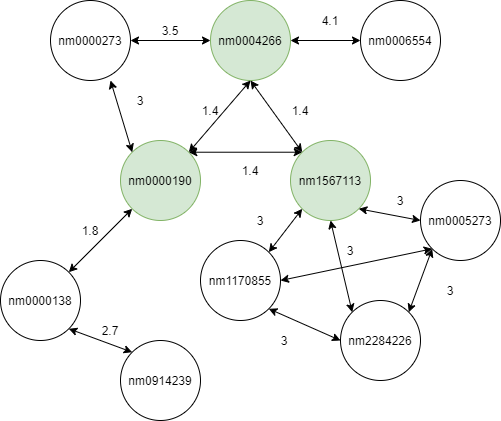
\includegraphics[width=\linewidth]{relation_graph.png}
    \justifying
    \small
    For the Use case example (Interstellar): Matthew McConaughey: nm0000190, Anne Hathaway: nm0004266, Jessica Chastain: nm1567113 are the main actors. The edges represent the average of the inverse distance and the inverse rating.
    \caption{A sample snapshot of the actor-actor relationship graph}
    \label{fig: relation graph}
\end{figure}



Since we have not been able to find a description of a multi start and end node breadth first algorithm we would like to include a description of it. The first iteration of our algorithm is the normal breadth first algorithm. The graph is stored in a DataFrame, and the current paths are stored in another DataFrame. Start by taking the starting node and adding it and every edge from it to the DataFrame. Continue adding edges to the DataFrame n times, where n is the number of steps you are using. The resulting DataFrame should have several columns where the first one is the starting node, the following columns should be the edge and cost to that edge. By applying a function to each row of the DataFrame we can calculate the cost from the starting node to the last edge node following the path along every edge in that row. If the goal node is found along the path, then we return the cost, otherwise a token value is returned. The token value should be outside of the cost function domain or be on an extreme of the domain meaning that in any situation it will not be considered as a possible path to the goal node. In our case, we use a token value of -1 because the domain of our cost function is [0, 10]. The inverse of the cost function is returned and stored in a score column. Finally, the score column is aggregated to find the maximum and this is returned as the relation score between the two actor nodes. By observing that calculating the path from A-B-C is done by a 2-step search from A, is done no matter what our goal node is. The algorithm can be improved by allowing a list of goal nodes. When applying the cost function simply check if any of the goal nodes are found along the path. This is a simple change that improves the exeuction time a lot. If you look at the score between one actor and 8 other actors, the exeuction time is about 20 seconds for each relation if you are using the breadth first algorithm. With the multi goal optimisation, the time is reduced to about 2.5 seconds for each relation. When calculating the relation scores between the candidate lists A and B of size 30 each, the number of function calls is now reduced from 90 to just 30. A simplified version of this function is shown in code listing \ref{CodeBFS}.



\begin{lstlisting}[float=h, language=Python, caption=Simplified multi-start to multi-goal search algorithm, label=CodeBFS, numbers=left]
# Get initial nodes and their edges
current = graph.filter(F.col("node").isin(start_nodes))
current = current.join(graph, current.node == graph.node)
# Do n steps
for i in range(1, n):
    current = current.select("*", F.explode(current.edges))
    current = current.join(graph, current.last_node == graph.node)
# Split by starting node and find best score
current = current.withColumn("score", calculate_score(current.columns))
current = current.select("start", F.explode(F.col("score")).alias("goal", "score"))
best_scores = current.groupby(["start", "goal"]).max("score").collect()
return best_scores
\end{lstlisting}



By observing that the same calculations are done when finding the path from A1 to B and A2 to B we can improve it further to a multi start node algorithm. The most expensive part of the algorithm is transferring the graph edges to the current path. The number of times we do this grows with the number of times we call the merge function on two dataframes. By looking at the path from multiple start nodes to multiple goal nodes the number of merges is reduced and the number of function calls can be reduced to 1. 

Following the assumptions from before, the total time for a 2-step search is 129 seconds. This gives a time per relation of 0.048 seconds which means that compared to the original algorithm, the execution time has been improved by a factor of 9500. The number of paths for the 3-step search is quite a bit larger but the improvement is still significant. The total execution time is 4402 seconds, giving a time per relation of 1.63 seconds which is a 280 times improvement. 


\begin{lstlisting}[float=h!, language=Python, caption=Calculating group scores using PySpark, label=CodeUDF, numbers=left]
    @F.udf("float")
    def calc_final_score(row):
        actors = row[0].split(", ")
        relation_scores = []
        # Retrieve every actor to actor relation score.
        for i in range(len(actors)):
            for j in range(i + 1, len(actors)):
                relation_scores.append(relations[actors[i]][actors[j]])
        not_none = [score for score in relation_scores if score != None]
        n_not_none = len(not_none)
        if n_not_none == 0:
            return row[1]
        # Compute the relation score weighting based on how many relationships exist in the group.
        relation_ratio = (1 / 3) * n_not_none / len(relation_scores)
        # Return the final score as a weighted average.
        return (1 - relation_ratio) * row[1] + relation_ratio * sum(not_none) / n_not_none
    \end{lstlisting}

\subsubsection{Overall score}

The ranking algorithm is used to determine whether one actor could perform better than another. This is done by calculating a score for the actors, before combining them to get a score for the whole group. Our algorithm assumes the first actor description to be the primary actor and tries to maximise the cast rank based on this. The following is a description of our algorithm. The first step is to find every actor that matches the primary actor description. For every matching actor, a score is calculated. It is a combination of the genre score, past acting relationship (maybe) and how similar the plots of the movies the actor has acted in are to the user plot. The genre score is taken as the average of the actor genre scores, given that they match the user genres. This is done because one actor might have a high score in war and action movies, but low in romance and drama. If the user is making a romance and drama movie, then the genre score is taken as the average of just those two scores. The plot of every movie the actor has been in is compared to the user plot. The maximum similarity score is used for the actor score. To make the average of the genre score and the similarity equally important for the actor score the similarity bound is changed to (0, 10). Then the actor score is changed to be in the interval (0, 1). Thus the expression for the score is: $actor(id)=\frac{1}{20}(avg(genrescore)+5.(max(similarity)+1))$.To find the other actors the procedure above is repeated on the actors matching the other descriptions. Because we consider it beneficial to cast actors who have worked together before, we use the relation score calculation stated above to calculate the actor relation score. To calculate the cast score, we also make a prediction of the IMDB rating that the resulting movie will have if the selected actors are in it. The prediction is calculated from the average of the actors’ average genre scores. The expression for the cast score is: $$cast(ids)=\frac{1}{\#ids}\sum_{i=1}^{\#ids}worked(ids_i, ids_1)\cdot actor(ids_i) + rating(ids)$$. The $worked$ function returns X if they have worked together before, 0 otherwise. The calculation is done using a user-defined function operating on each row, shown in listing \ref{CodeUDF}.

The cast score is used to rank the groups. A higher score means a better group. The groups are sorted in descending order and returned to the user.



\subsection{Workflow}

The summary of the workflow for our project is pictorially represented in the two figures. The Python process is described in \ref{fig:python-process}, and the Spark process is described in figure \ref{fig:spark-process}. As is shown in the figures the flow is very similar. The main difference is that the Spark version has a helper script to run the search which makes sure all of the data is loaded propery and available in the Spark context. The reason they are so similar is because that makes it easier to run comparisons and justify why it is valid to compare the result. The pre-preprocessing however is quite different because the Python version stores to users disk, while the Spark implementation uses the Hadoop cluster HDFS to store the data.

\begin{figure}[t]
	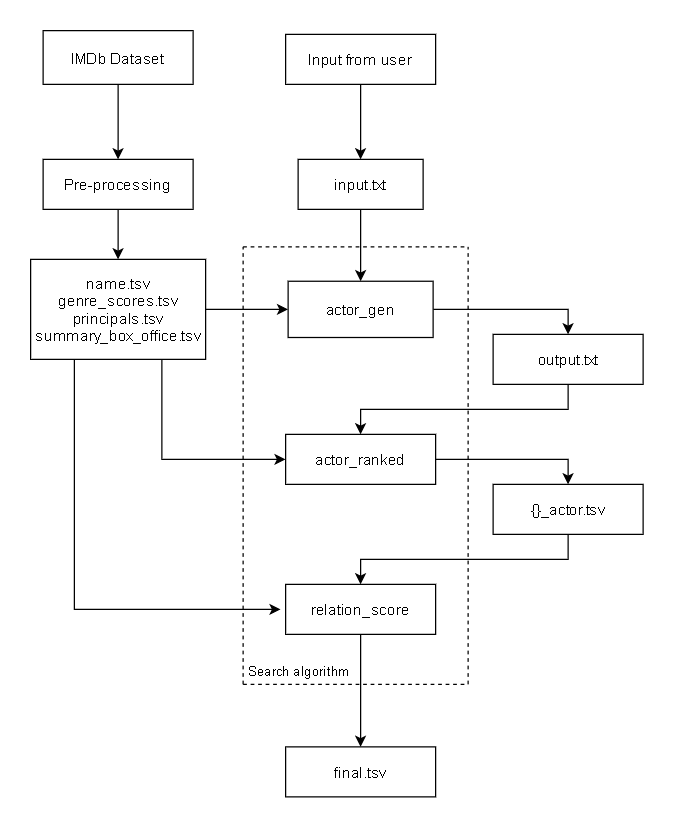
\includegraphics[width=8.25cm,keepaspectratio]{python_workflow.png}
	\caption{Python process workflow}
	\label{fig:python-process}
\end{figure}


\begin{figure}[t]
	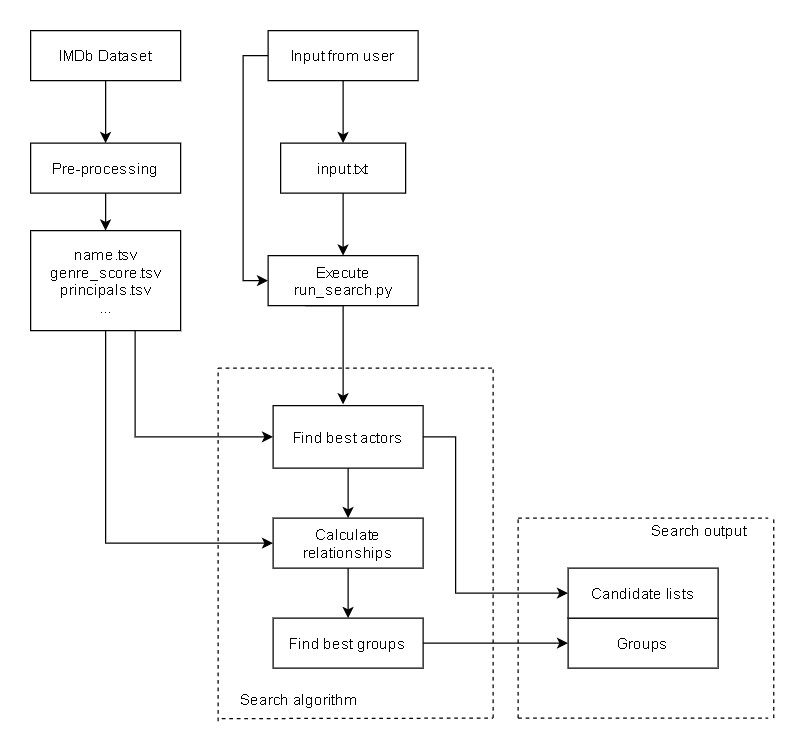
\includegraphics[width=8.25cm,keepaspectratio]{spark_workflow.png}
	\caption{Spark process workflow}
	\label{fig:spark-process}
\end{figure}



\subsection{Algorithm results}

The runtime of our algorithm is not the only evaluation we need to base our efficiency on. The result of a search is equally or more important. We first need to define what a good result is, and then how we decide whether or not a result is better than another. The obvious answer to what a good result is, is one that maximises the scores discussed in the previous sections. Following from that answer we also need to justify why those are good methods of measuring an actors’ ability to perform well. We think it is intuitively true that if an actor has performed well earlier, they are more likely to perform well in their next movie of the same genre than someone who has a comparatively bad acting history. The same can be said about the similarity score, if someone has acted in a similar movie before then they are likely familiar with the setting and mindset they need to be in while acting. This does not however hold when arguing why the relationship score is relevant. Our reasonable justification for this is that we believe the assumption: "Any movie with a high user rating on IMDb has a good cast" to be true. From this we can say that if two actors have acted together in a movie with a high rating then they are good at acting together, and the opposite if the movie has a low rating then they should probably not act together. This assumption also means that we should have the following goal for our search engine: if you do a search with the attributes from a movie on IMDb, the original cast should be early in the result if the movie has a high rating. There is a fallacy to be aware of here. If you only try to achieve this goal, for example by weighing the similarity score and the relationship score by a large constant, then the individual is lost and the engine will most likely only return previous movie casts for any new query. 

We believe we found a good balance between the importance of the different scores. A problem with the result we discovered while working on the engine is that when combining individual actors into groups then you need to have some measure of their relationship to avoid having the groups be a combination of just the individually best actors. What we mean by this is that if A and B actors have a sufficiently large score then they will be the suggested for several of the top groups, for example ABC, ABD, ABE, ABF and so on. This is of course the correct result based on the score, but it does not give a lot of information to the user because they are suggested a low number of actors relative to the number of groups. E.g. five groups make it possible to have 15 distinct actors, but the actual result might only contain 7 actors if the two first candidates are constant. This problem was our main motivation behind adding the relationship score. While it did help alleviate the problem, we still feel like this is a major problem with our search engine. To improve the result we decided to include the top ranked candidates from each list together with the top groups such that if the user feels like some actors are repeated too often then they can look at the individual lists for other alternatives.
